\documentclass[a4paper, 11pt]{article}

%%%%导入包%%%%

\usepackage{xeCJK}
\usepackage{algorithm}
\usepackage{algorithmic}
\usepackage{graphicx}
\usepackage[unicode]{hyperref}
\usepackage{xcolor}
\usepackage{cite}
\usepackage{indentfirst}
\usepackage{amsfonts}
\usepackage{amsmath}
\usepackage{amssymb}
\usepackage{amsthm}
\usepackage{multirow}

%\usepackage{ctex}

\setCJKmonofont{SimHei}  %设置等宽字体
\setCJKsansfont{KaiTi}  %设置楷体
\setCJKmainfont{KaiTi}  %设置缺省中文字体 楷体
\setCJKmonofont{SimHei}  %设置等宽字体
\setmainfont{Arial} % 英文衬线字体
\setmonofont{Arial} % 英文等宽字体
\setsansfont{Arial} % 英文无衬线字体

\setCJKfamilyfont{somefont}{SimHei}
\newcommand*{\somefont}{\CJKfamily{somefont}} 

%%%%%% 设置字号 %%%%%%
\newcommand{\chuhao}{\fontsize{42pt}{\baselineskip}\selectfont}
\newcommand{\xiaochuhao}{\fontsize{36pt}{\baselineskip}\selectfont}
\newcommand{\yihao}{\fontsize{28pt}{\baselineskip}\selectfont}
\newcommand{\erhao}{\fontsize{21pt}{\baselineskip}\selectfont}
\newcommand{\xiaoerhao}{\fontsize{18pt}{\baselineskip}\selectfont}
\newcommand{\sanhao}{\fontsize{15.75pt}{\baselineskip}\selectfont}
\newcommand{\sihao}{\fontsize{14pt}{\baselineskip}\selectfont}
\newcommand{\xiaosihao}{\fontsize{12pt}{\baselineskip}\selectfont}
\newcommand{\wuhao}{\fontsize{10.5pt}{\baselineskip}\selectfont}
\newcommand{\xiaowuhao}{\fontsize{9pt}{\baselineskip}\selectfont}
\newcommand{\liuhao}{\fontsize{7.875pt}{\baselineskip}\selectfont}
\newcommand{\qihao}{\fontsize{5.25pt}{\baselineskip}\selectfont}

%%%% 设置 section 属性 %%%%
\makeatletter
\renewcommand\section{\@startsection{section}{1}{\z@}%
{-1.5ex \@plus -.5ex \@minus -.2ex}%
{.5ex \@plus .1ex}%
{\normalfont\sihao\CJKfamily{hei}}}
\makeatother

%%%% 设置 subsection 属性 %%%%
\makeatletter
\renewcommand\subsection{\@startsection{subsection}{1}{\z@}%
{-1.25ex \@plus -.5ex \@minus -.2ex}%
{.4ex \@plus .1ex}%
{\normalfont\xiaosihao\CJKfamily{hei}}}
\makeatother

%%%% 设置 subsubsection 属性 %%%%
\makeatletter
\renewcommand\subsubsection{\@startsection{subsubsection}{1}{\z@}%
{-1ex \@plus -.5ex \@minus -.2ex}%
{.3ex \@plus .1ex}%
{\normalfont\xiaosihao\CJKfamily{hei}}}
\makeatother

%%%% 段落首行缩进两个字 %%%%
\makeatletter
\let\@afterindentfalse\@afterindenttrue
\@afterindenttrue
\makeatother
\setlength{\parindent}{2em}  %中文缩进两个汉字位

%%%% 下面的命令重定义页面边距,使其符合中文刊物习惯 %%%%
\addtolength{\topmargin}{-54pt}
\setlength{\oddsidemargin}{0.63cm}  % 3.17cm - 1 inch
\setlength{\evensidemargin}{\oddsidemargin}
\setlength{\textwidth}{14.66cm}
\setlength{\textheight}{24.00cm}    % 24.62

%%%% 下面的命令设置行间距与段落间距 %%%%
\linespread{1}
% \setlength{\parskip}{1ex}
\setlength{\parskip}{0.3\baselineskip}

%%%% 正文开始 %%%%
\begin{document}

%%%% 定理类环境的定义 %%%%
\newtheorem{example}{例}             % 整体编号
%\newtheorem{algorithm}{算法}
\newtheorem{theorem}{定理}[section]  % 按 section 编号
\newtheorem{definition}{定义}
\newtheorem{axiom}{公理}
\newtheorem{property}{性质}
\newtheorem{proposition}{命题}
\newtheorem{lemma}{引理}
\newtheorem{corollary}{推论}
\newtheorem{remark}{注解}
\newtheorem{condition}{条件}
\newtheorem{conclusion}{结论}
\newtheorem{assumption}{假设}

%%%% 重定义 %%%%
\renewcommand{\contentsname}{目录}  % 将Contents改为目录
\renewcommand{\abstractname}{摘要}  % 将Abstract改为摘要
\renewcommand{\refname}{参考文献}   % 将References改为参考文献
\renewcommand{\indexname}{索引}
\renewcommand{\figurename}{图}
\renewcommand{\tablename}{表}
\renewcommand{\appendixname}{附录}
%\renewcommand{\algorithm}{算法}

\title{Partial Annotation based CRF}
\author{朱运}

\maketitle

\section{符号定义}

$\mathcal{D}=\{S^j,Y^j\}_{j=1}^N$:表示一个数据集,包含$N$个句子和对应的$N$个人工标注的分词序列。

$S^j=w_1^j...w_i^j...w_{n_j}^j$:表示第$j$个句子,由$n_j$个汉字组成。

$Y^j=y_1^j...y_i^j...y_{n_j}^j$:表示第$j$个句子对应的标签序列。

$\mathcal{T}$:表示标签集合,即隐状态的所有可能取值,$y_i^j \in \mathcal{T}$。

$\mathcal{V}$:表示字表(vocabulary),即数据$\mathcal{D}$所有汉字的集合,$w_i^j \in \mathcal{V}$。

\section{ 概念定义}

%全标注就是$Y^j$这个标签序列里面每一个位置的tag集合是$\mathcal{T}$子集,且集合里面只有一个tag。
以汉语分词任务举例,对于一个例句“我是中国人。”,我们采用四标签集(BMES),B、M、E、S分别代表一个词的开始,中间,结尾和单字成词。

全标注是指句子中的每个字都给出了正确的分词标签,即 |$Y^j$| = |$S^j$|。假设全标注对应的tag序列是Y =(S,S,B,M,E,S),如图1所示,那么其每个汉字对应的tag集合就是(\{S\},\{S\},\{B\},\{M\},\{E\},\{S\})

\begin{figure}[htbp]
  \centering
  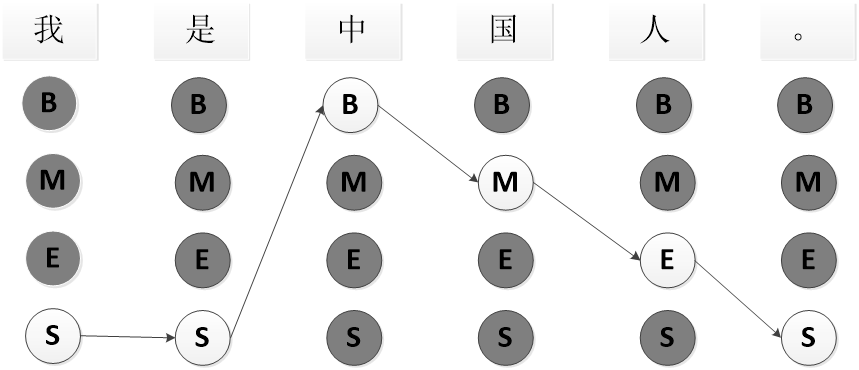
\includegraphics[width=0.8\textwidth]{full_anno_pic.png}
  \caption{全标注}\label{fig:digit}
\end{figure}

\newpage

%局部标注就是$Y^j$这个标签序列里面只有给定位置的tag集合是$\mathcal{T}$子集且只有一个tag,其余位置的tag集合是$\mathcal{T}$。
部分标注是指句子只有某些字的分词标签给出了,而其余的字的标签没有给出,我们可以将全标注作为局部标注的一种特殊情形。假设部分标注已知的切分信息是“中国人”是一个词,其余位置未知,那么“中国人”对应的tag序列是(B,M,E),如图2所示,那么其每个汉字对应的tag集合就是(\{B、M、E、S\},\{B、M、E、S\},\{B\},\{M\},\{E\},\{B、M、E、S\})
\newline
\newline
\begin{figure}[htbp]
  \centering
  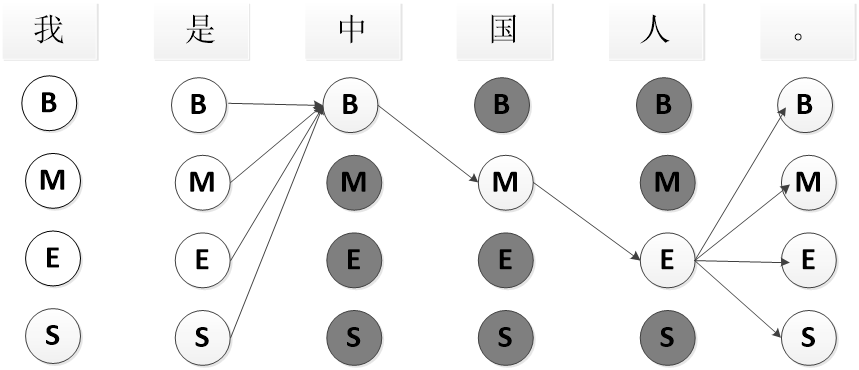
\includegraphics[width=0.8\textwidth]{partial_anno.png}
  \caption{部分标注}\label{fig:digit}
\end{figure}
\newline
\newline

%模糊标注就是$Y^j$这个标签序列里面只有给定位置的tag集合是$\mathcal{T}$子集且集合里面不只有一个tag,其余位置的tag集合就是$\mathcal{T}$。
这里,我们定义了 模糊标注:即句子中,每个字的标签是不唯一的,即我们允许一个字可以有多个标签。假设模糊标注已知的切分信息是“中国人”或者“中国”和“人”,其余位置未知,如图3所示,那么其每个汉字对应的tag集合就是(\{B、M、E、S\},\{B、M、E、S\},\{B\},\{M、E\},\{E、S\},\{B、M、E、S\})
\newline
\newline
\begin{figure}[htbp]
  \centering
  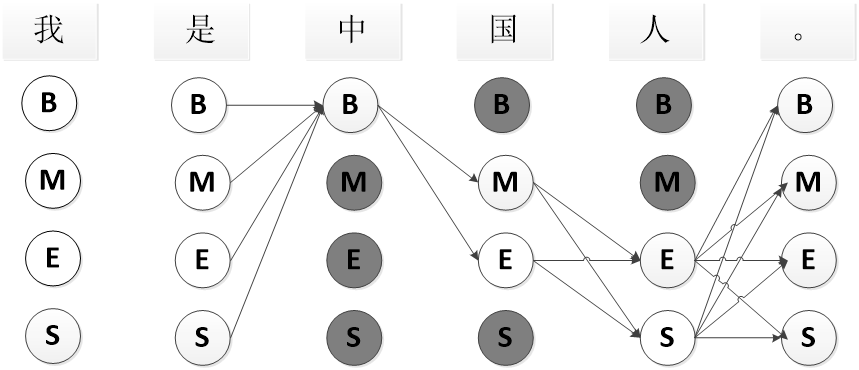
\includegraphics[width=0.8\textwidth]{mohubiaozhu.png}
  \caption{模糊标注}\label{fig:digit}
\end{figure}
\newline
\newline

\section{ 公式推导}
我们采用CRF模型来处理分词的序列标注问题。给定一个输入的字符序列,模型的作用是给这个序列每个位置的字赋予对应的一个标签。

\newpage
全标注中,假设给定的一个句子S = $w_1$...$w_n$,其对应的正确tag序列为Y = $y_1$...$y_n$。 
那么CRF定义句子$S$标注为序列$Y$的概率为:

\begin{equation} \label{eq:CRF_probability}
\begin{split}
p(Y|S) = \frac{e^{\textit{Score}(S, Y)}}{Z(S)} \\
\end{split}
\end{equation}

其中

\begin{equation} \label{eq:zx}
\begin{split}
Z(S) = \sum_{Y' \in \mathcal{T}^n}e^{\textit{Score}(S, Y')} \\
\end{split}
\end{equation}

部分标注中,如图2所示,只有句子里面给定的词有固定的tag,其余位置标签不确定,那么符合图2情况的序列集合

$Y_L$ = \{(B,B,B,M,E,B),(M,B,B,M,E,B),(E,B,B,M,E,B),(S,B,B,M,E,B),

\indent\hspace{0.9cm}	(B,M,B,M,E,B),(M,M,B,M,E,B),(E,M,B,M,E,B),(S,M,B,M,E,B),

\indent\hspace{0.9cm}	(B,E,B,M,E,B),(M,E,B,M,E,B),(E,E,B,M,E,B),(S,E,B,M,E,B),

\indent\hspace{0.9cm}	(B,S,B,M,E,B),(M,S,B,M,E,B),(E,S,B,M,E,B),(S,S,B,M,E,B)...\}

\noindent 集合里面一共4*4*1*1*1*4 = 64种情况。其中$Y_L$表示所有可能的序列集合,那么$Y_L$的边缘概率可以表示为


\begin{equation} \label{eq:CRF_partial_probability}
\begin{split}
p(Y_L|S) = \sum_{y \in {Y_L} }\frac{e^{\textit{Score}(S, y)}}{Z(S)} \\
\end{split}
\end{equation}

我们定义${Z_L}$为:
\begin{equation} \label{eq:CRF_partial_Z_probability}
\begin{split}
Z_{Y_L} = \sum_{y \in {Y_L} }{e^{{Score}(S, y)}} \\
\end{split}
\end{equation}

那么部分标注的边缘概率就可以归一化为:
\begin{equation} \label{eq:CRF_normal_partial__probability}
\begin{split}
p(Y_L|S) =  \frac{Z_{Y_L}}{Z(S)} \\
\end{split}
\end{equation}

根据全标注的CRF似然函数
\begin{equation} \label{eq:ll}
\begin{split}
LL(\mathcal{D};\mathbf{w}) &= \sum_{j = 1}^N \left [ \textit{Score}(S^j, Y^j) - \mathrm{log}Z(S^j)\right  ]  \\						  
\end{split}
\end{equation}


我们可以得到对应的部分标注的似然函数:
\begin{equation} \label{eq:partial_ll}
\begin{split}
LL(\mathcal{D};\mathbf{w}) &= \sum_{j = 1}^N \left [\mathrm{log}Z_{Y_L}(S^j) - \mathrm{log}Z(S^j)\right ]  \\                                               
\end{split}
\end{equation}

根据CRF似然函数求解:
\begin{equation} \label{eq:logz-partial}
\begin{split}
\frac{\partial{\mathrm{log}Z(S^j)}}{\partial{\mathbf{w}}} &= \sum_{Y' \in \mathcal{T}^n} p(Y'|S)\cdot \mathbf{f}(S^j, Y') \\
\end{split}
\end{equation}

可以得到:
\begin{equation} \label{eq:logZ_Y_L-partial}
\begin{split}
\frac{\partial{\mathrm{log}Z_{Y_L}(S^j)}}{\partial{\mathbf{w}}} &= \sum_{Y' \in Y_L} p(Y'|S)\cdot \mathbf{f}(S^j, Y') \\
\end{split}
\end{equation}

$Z_{Y_L}$和{Z}的形式以及计算梯度方式很相似,通过对$Z_{Y_L}$的前向alpha和后向beta的计算加上一些约束,我们可以将$Z_{Y_L}$和Z的计算统一起来。
\begin{equation} \label{eq:alpha_z_y_l}
\begin{split}
\alpha_{Z_{Y_L}}(k, t) &=\left\{
\begin{array}{lcl} \sum_{(t',t) \in {Y_L}}e^{\textit{Score}(S, k, t', t)}\cdot \alpha(k - 1, t')	&	&{ (t', t) \in {Y_L}} \\
			    0		&	& {(t', t) \notin {Y_L}} 
\end{array} \right.
\end{split}
\end{equation}

\begin{equation} \label{eq:beta_z_y_}
\begin{split}
\beta_{Z_{Y_L}}(k, t) &=\left\{
\begin{array}{lcl} \sum_{(t,t') \in {Y_L}}e^{\textit{Score}(S, k + 1, t, t')}\cdot \beta(k + 1, t')		&	&{ (t,t') \in {Y_L}} \\
				0		&	& {(t,t') \notin {Y_L}} 
\end{array} \right.
\end{split}
\end{equation}


同理,模糊标注的计算方式和局部标注的计算一样。



\section{说明}
全标注,部分标注以及模糊标注在训练和测试的时候不需要考虑tag之间的约束关系(即标签B之后只能接标签E或者M,而不能接标签S),只有在算prf值需要解码的时候需要考虑tag之间的约束关系。










\end{document}































